\subsection{Universidad de Helsinki}

Resultados obtenidos en el monitoreo:\\

\smallskip
\begin{tabular}{| l | c | c | c | c |}
\hline
Hop & IP &  RTT promedio (s)  & deltaRTT promedio & Ubicacion\\ 
\hline
1 & 192.168.11.1 & 0.01142361429 & 0.01142361429 & Argentina, Buenos Aires\\
\hline
2 & 10.21.128.1 & 0.0283621417152 & 0.0169385274251 & Argentina, Buenos Aires\\
\hline
3 & 10.242.0.201 & 0.0378749105665 & 0.00951276885139 & Argentina, Buenos Aires\\
\hline
4 & 195.22.220.33 & 0.0143795543247 & 0 & Italy\\
\hline
5 & 195.22.220.32 & 0.292960882187 & 0.278581327862 & Italy\\
\hline
6 & 89.221.41.171 & 0.152727180057 & 0 & Italy\\
\hline
7 & 89.221.41.171 & 0.156960460875 & 0.00423328081767 & Italy\\
\hline
8 & 154.54.9.17 & 0.202791770299 & 0.0458313094245 & United States\\
\hline
9 & 154.54.80.41 & 0.21254154614 & 0.00974977584112 & United States\\
\hline
10 & 66.28.4.237 & 0.168935351902 & 0 & United States, Pasadena\\
\hline
11 & 154.54.29.222 & 0.251122385263 & 0.0821870333619 & United States\\
\hline
12 & 154.54.42.77 & 0.316137870153 & 0.0650154848893 & United States\\
\hline
13 & 154.54.45.162 & 0.327892038557 & 0.0117541684045 & United States\\
\hline
14 & 154.54.45.2 & 0.255609459347 & 0 & United States\\
\hline
15 & 38.88.196.186 & 0.270633061727 & 0.0150236023797 & United States, Los Angeles\\
\hline
16 & 101.4.117.169 & 0.435372935401 & 0.164739873674 & China, Beijing\\
\hline
17 & 101.4.117.97 & 0.467933893204 & 0.0325609578027 & China, Beijing\\
\hline
18 & 101.4.112.105 & 0.437322590086 & 0 & China, Beijing\\
\hline
19 & 101.4.118.94 & 0.43985332383 & 0.0025307337443 & China, Beijing\\
\hline
20 & 101.4.112.90 & 0.435603486167 & 0 & China, Beijing\\
\hline
21 & 101.4.117.81 & 0.413042836719 & 0 & China, Beijing\\
\hline
22 & 202.112.41.178 & 0.405184189479 & 0 & China, Shanghai\\
\hline
23 & 202.112.41.182 & 0.394645796882 & 0 & China, Shanghai\\
\hline
24 & 162.105.252.133 & 0.488684309853 & 0.0940385129717 & China, Beijing\\
\hline
\end{tabular}
\bigskip

\textbf{Paquetes enviados: 407 / Paquetes no respondidos: 37}\\

\textbf{Tres outliers, hops: 4, 6 y 8}\\

En el mapa se puede observar que hay un enlace intercontinental entre Argentina e Italia, el cuál es detectado correctamente por el método Cimbala (hop 4). Sin embargo, vuelve a detectar un outlier en el hop 6, el cual sigue estando en Italia. Creemos que este hop fue detectado como un outlier debido a la gran diferencia entre el RTT de ese hop y el del hop anterior, como se puede observar en el gráfico de RTTs relativos. También detecta un enlace submarino desde Italia hasta Suecia (hop 8).
En este caso consideramos que el método Cimbala para detectar outliers funcionó correctamente, ya que los outliers detectados son de interés.


A continuación mostramos un gráfico con los RTT entre saltos y otro con los ZRTT\footnote{ZRTT = $(X_i - \bar{X}) / S$}  entre saltos. También así el planisferio con los saltos graficados.

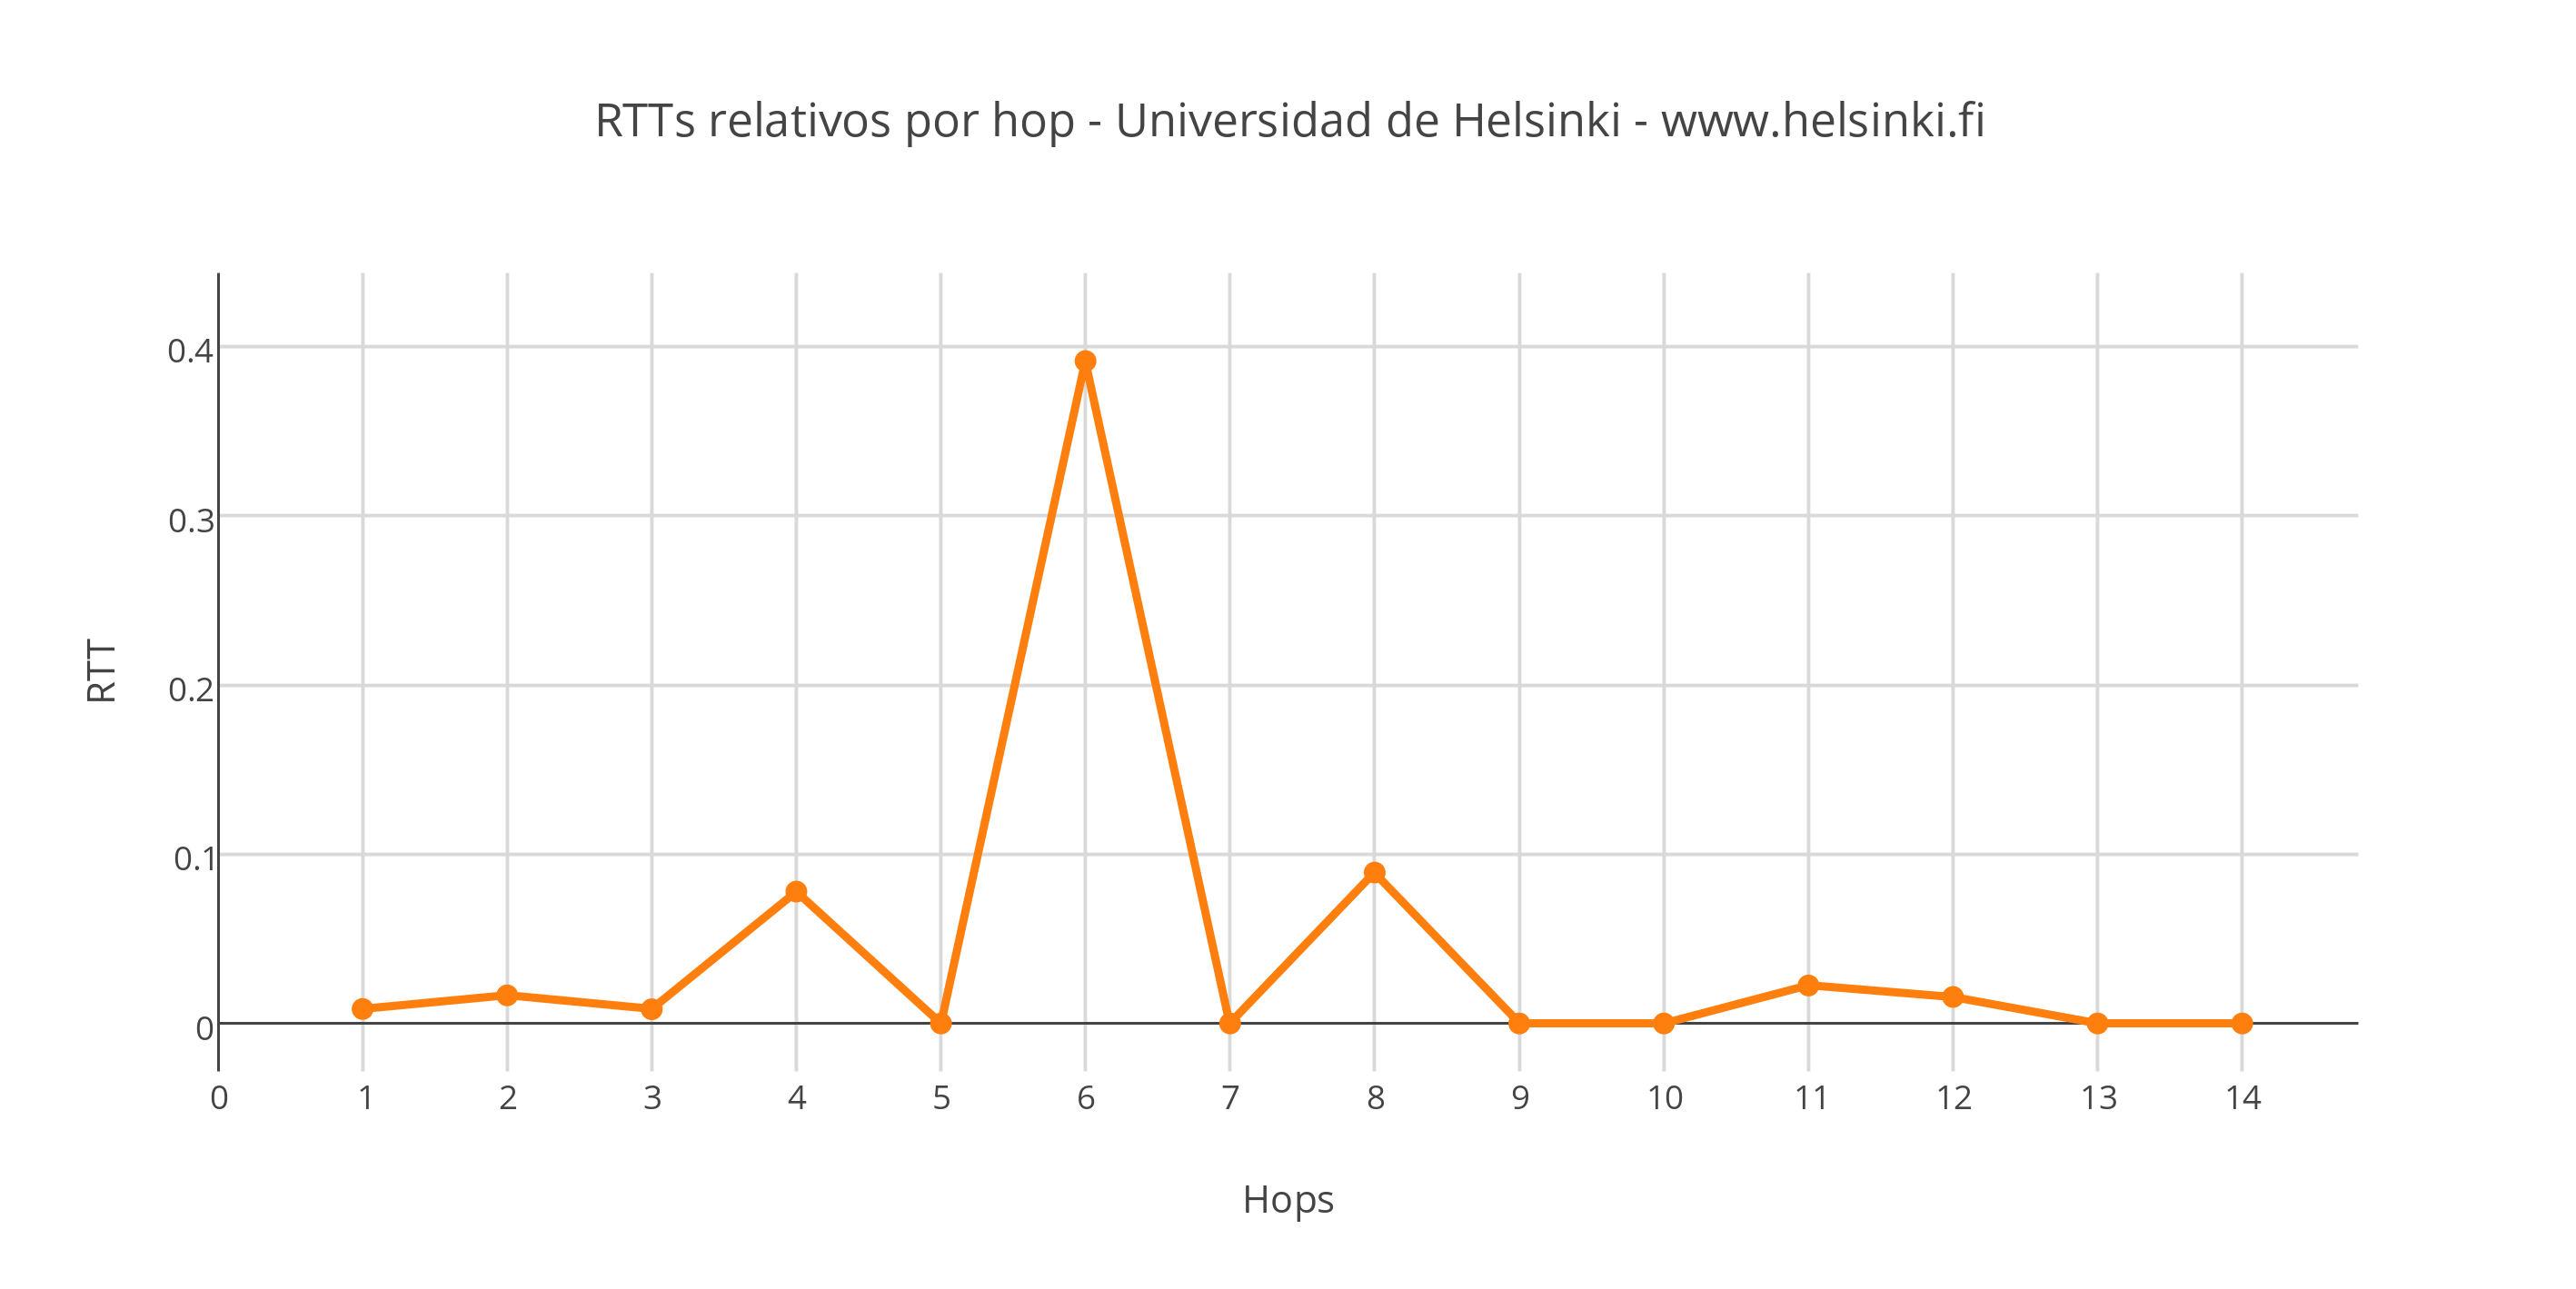
\includegraphics[scale=0.65]{imagenes/helsinki/RTTs.png} 

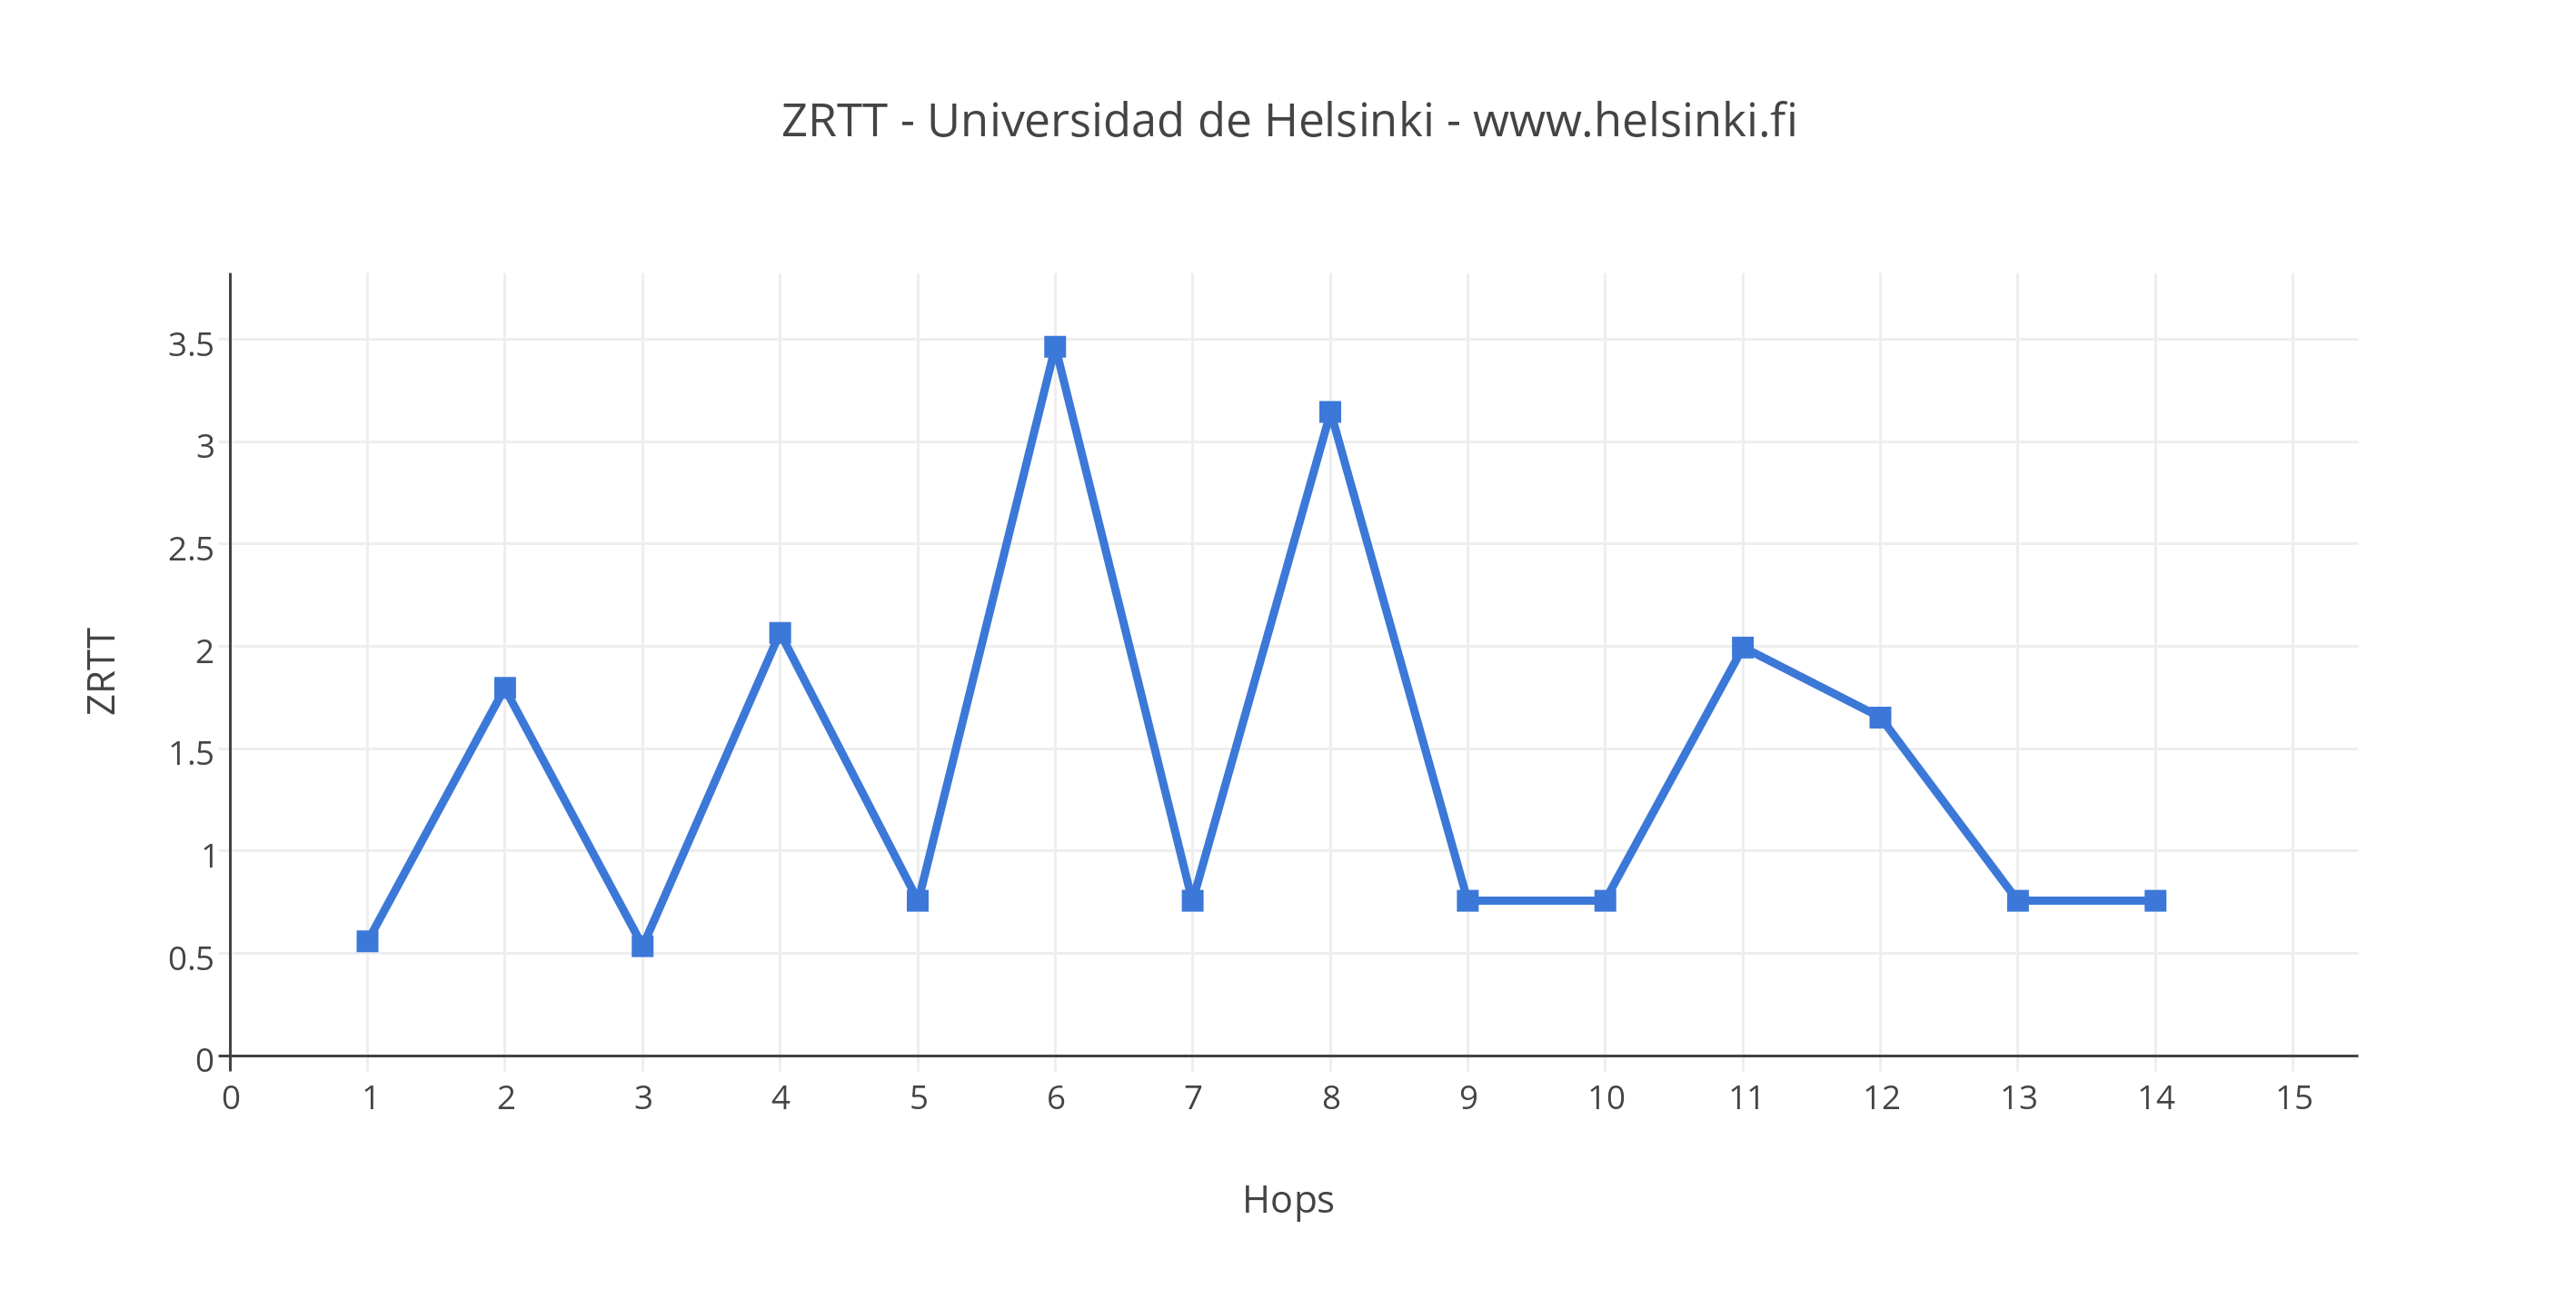
\includegraphics[scale=0.65]{imagenes/helsinki/ZRTTs.png} 

\begin{center}
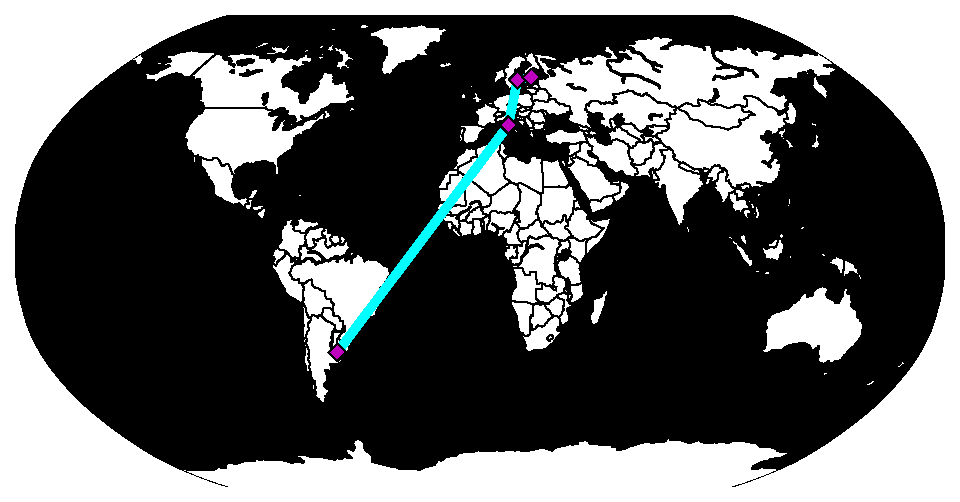
\includegraphics[scale=0.8]{imagenes/helsinki/helsinki.pdf} 
\end{center}